\section{Concept 3 - Trade-off}
\begin{figure}[!htbp]
  \centering
  \subbottom[Actors tab\label{sfig:customer-ui-mockup-actors}]{%
    \includegraphics[width=0.49\linewidth]{\imgdir customer-ui-mockup-actors}}
  \subbottom[Uses cases tab\label{sfig:customer-ui-mockup-use-cases}]{%
    \includegraphics[width=0.49\linewidth]{\imgdir customer-ui-mockup-use-cases}}
    
  \subbottom[Definitions tab\label{sfig:customer-ui-mockup-definitions}]{%
    \includegraphics[width=0.49\linewidth]{\imgdir customer-ui-mockup-definitions}}
  \caption{Mock-up screens of the customer user interface.}
\end{figure}
\begin{figure}[!htbp]
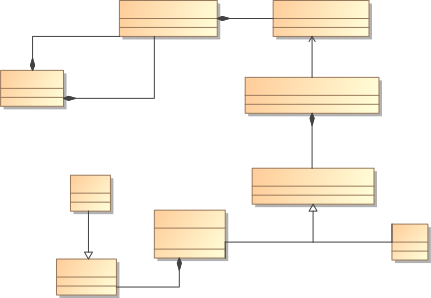
\includegraphics[scale=0.9]{img/3rd_iteration_meta_model}
\centering
\caption{Meta model of the third concept}
\label{fig:3rd_iteration_meta_model}
\end{figure}

\subsection{Definition}
A definition is textual description of a concept which may be -- for instance -- an actor, role or action. This description is then given a unique name, that may correspond to a concept already found in the domain model. The domain model, if defined beforehand, could also be thought to be a part of the built-in declarations.
